\documentclass{article}
\usepackage[utf8]{inputenc}

% Page setup
\usepackage[a4paper,landscape,margin=2cm]{geometry}
\usepackage{amsmath}

% Typography
\usepackage[scaled]{helvet}
\let\familydefault\sfdefault

\usepackage[usenames,svgnames]{xcolor}
\usepackage{tikz,pgfplots}
\usetikzlibrary{positioning,arrows,intersections}

\definecolor{colordict}     {RGB}{143,232,186}
\definecolor{colortext}     {RGB}{29 ,29 ,27 }

\begin{document}
\pagestyle{empty}
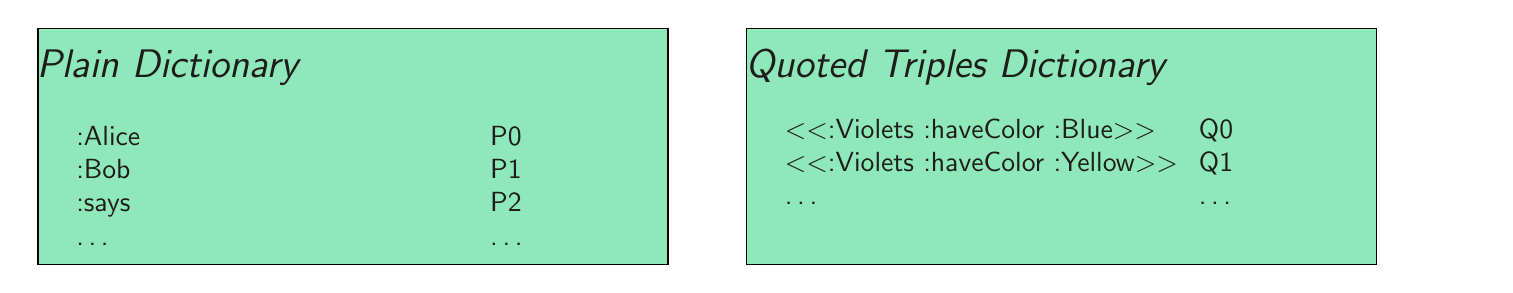
\begin{tikzpicture}[
    node distance = 5em, auto,
    font={\Large\itshape},
    title/.style={text=colortext,font={\Large\itshape}},
    code/.style={text=colortext,font={}},
]

    \draw[fill=colordict] (0,0) rectangle (8,3);
    \node[title,text width=20em] at (3.5,2.5) {Plain Dictionary};
    \node[code,text width=20em] at (4,1) {:Alice\\
    :Bob\\
    :says\\
    \ldots};
    \node[code,text width=10em] at (7.5,1) {P0\\
    P1\\
    P2\\
    \ldots};
    
    \draw[fill=colordict] (9,0) rectangle (17,3);
    \node[title,text width=20em] at (12.5,2.5) {Quoted Triples Dictionary};
    \node[code,text width=20em] at (13,1.3) {$<<$:Violets :haveColor :Blue$>>$\\
    $<<$:Violets :haveColor :Yellow$>>$\\
    \ldots};
    \node[code,text width=10em] at (16.5,1.3) {Q0\\
    Q1\\
    \ldots};

\end{tikzpicture}
\end{document}
